
\documentclass[runningheads]{llncs}
%
\usepackage{graphicx}
% Used for displaying a sample figure. If possible, figure files should
% be included in EPS format.
%
\usepackage{hyperref}
\usepackage{color}
% If you use the hyperref package, please uncomment the following line
% to display URLs in blue roman font according to Springer's eBook style:
\renewcommand\UrlFont{\color{blue}\rmfamily}

% For image caption
\usepackage{caption}
\usepackage{subcaption}

\begin{document}
%
\title{DETECTION OF CIPHER TYPES USING ARTIFICIAL NEURAL NETWORKS
}
%
\titlerunning{DETECTION OF CIPHER TYPES USING ANN}
% If the paper title is too long for the running head, you can set
% an abbreviated paper title here
%
% \author{Malay Kule et al.\inst{1}}

\author{Malay Kule\inst{1}\and
Krishnendu Bera\inst{1}\and
Abhiroop Mukherjee\inst{1}\and
Arnab Sen\inst{1}\and
Swarnali Mondal\inst{1}\and
Sanjana Chakravarty\inst{1}\and
Rajdeep Ghosh\inst{1}}
%
\authorrunning{Malay Kule et al.}
% First names are abbreviated in the running head.
% If there are more than two authors, 'et al.' is used.
%
\institute{Indian Institute of Engineering Science and Technology, Shibpur
\email{malay.kule@gmail.com}\\
%\url{http://www.springer.com/gp/computer-science/lncs}
}
%
\maketitle              % typeset the header of the contribution
%
\begin{abstract}
The identification of a cryptosystem has been a challenge for decades. In this paper, the main objective is to identify the type of cryptosystem used to encrypt a certain piece of text. We have explored the realm of Artificial Neural Networks(ANNs) to recognize a pattern among complex classical cipher texts that generally have a simple representation in plain text. We have modelled our objective as a sequence-to-sequence learning task that we have tried to solve using Convolution Neural Networks (CNNs) and state-of-the-art Transformer models. With only a small dataset (130k) consisting of cipher texts and the corresponding cryptosystem used to encrypt the same, our model has shown a promising accuracy of 96.72 \% which proves a significantly steep learning curve as compared to other sequence-to-sequence models. Here we show the enormous potential of these models and how they can perform even better if the barrier of resources and computation time is lifted.


\keywords{ Artificial Neural Networks(ANNs)\and Cryptosystem Identification \and Classical Cipher text classification \and Convolution Neural Networks(CNNs) \and Transformer models.}
\end{abstract}
%
%
% Introduction section
\section{Introduction}
In today's world, information is a powerful tool. However, it is essential to protect information and data from unauthorized access, distortion, or any other unauthorized activity. Cryptography is the study of secret writing and is used to prevent unauthorized access to data. It works by using a key(s) to convert plaintext messages into unreadable ciphertext and vice versa. Encryption is the process of converting plaintext message into an unreadable format to protect sensitive information (called ciphertext), while the inverse process is called decryption. Only authorized users can encrypt or decrypt messages~\cite{katz2020introduction}.

The goal of the work is to use artificial neural networks to examine encrypted text files and classify them based on their cipher types. The process involves creating a collection of cipher texts with various cipher types, building a Deep Neural Network (DNN), and training it with a variety of cipher texts and training parameters to enable accurate learning and cipher text classification~\cite{inproceedings}. Once the DNN is trained, it can be used to determine the cipher text's kind. In this work, the Caesar, Affine, Vigenère, Substitution, and Rail Fence ciphers were used to encrypt English texts. The encrypted files were then submitted to CNN and Transformer models, which made predictions, and the accuracy of these predictions was assessed.

This paper is organized in four different sections. Section 2 describes the preliminaries for this work followed by this introductory section. Section 3 elaborates our proposed work with dataset generation and discussion of the models. Section 4 presents the experimental findings. The conclusion and the work that we intend to address in the future is contained in Section 5.

% Preliminaries section
\section{Preliminaries}
This paper requires basic knowledge of neural networks and deep learning, as well as an overview of the encryption algorithms used. These algorithms can be useful for feature extraction. The main machine-learning topics covered are artificial neural networks (ANN), perceptrons, recurrent neural networks (RNN), convolutional neural networks (CNN), and transformers.

\begin{itemize}

\item   \textbf{Artificial Neural Network (ANN)} – An artificial 
            neural network (ANN) is a type of computational model that mimics the human brain structurally and functionally~\cite{zupan1994introduction}. ANNs consist of layers of interconnected 
            neurons, which process input data and generate output 
            values. ANNs are trained to perform numerous types 
            of tasks, such as classification, regression, and clustering.

\item \textbf{Perceptron} – A perceptron is a type of artificial 
    neural network (ANN) that can be used for binary classification 
    tasks~\cite{gallant1990perceptron}. It consists of a single layer of neurons, with each neuron receiving input from multiple sources, and producing a single output value. A set of weights determines the output of a perceptron. Those weights are then applied to the input values, and a threshold value is used to determine whether the output is 0 or 1. 

\item \textbf{Convolutional Neural Network (CNN)} – CNNs 
    consist of multiple layers of interconnected neurons, which process 
    the input data in a hierarchical manner~\cite{DBLP:journals/corr/OSheaN15}. The first layer of a CNN typically consists of a set of filters. These filters are used extract features such as edges and textures by applying them to the input data. These features are then passed to the next layer of the CNN, where 
    they are combined and processed to extract more complex features, 
    such as shapes and objects. The output of a CNN is a set of 
    probabilities that indicate the likelihood that the input data 
    belongs to each of the possible classes.  
    
\item \textbf{Transformers} – The transformer is a type of encoder-decoder model, which is commonly used 
    for tasks such as machine translation and text summarization~\cite{vaswani2017attention}. 
    The key innovation of the transformer is the use of self-attention, 
    a mechanism that allows the model to learn dependencies 
    between different words in the input sentence. This allows 
    the transformer to process the input sentence in parallel, 
    rather than in a sequential manner, which makes it much 
    more efficient and scalable than previous NLP models.

\item \textbf{Attention Mechanism} – Self-attention is a 
    the mechanism used in the transformer ~\cite{vaswani2017attention}.With self-attention the model learns dependencies between different 
    words in the input, by computing weighted sum of the input 
    words based on their relevance to each other.

\end{itemize}
\section{Proposed Work}
\subsection{Dataset Generation}
The dataset has been generated for five types of ciphers:

\begin{itemize}
    \item Caesar
    \item Affine
    \item Vigenère
    \item Substitution
    \item Rail Fence
\end{itemize}

The plaintext used for encryption was the texts from Shakespeare’s Hamlet~\cite{2015haml65:online},  Macbeth~\cite{2015macb17:online}, Merchant of Venice~\cite{2015merc44:online} and Romeo and Juliet~\cite{2015rome60:online}.

We converted the text to lowercase and removed all whitespaces and punctuation. Then the plaintext was encrypted and exported as a CSV.

\subsection{CNN Based Proposed Model}  

The main intuition behind this method is that CNN uses its kernel as a “local receptive field”~\cite{DBLP:journals/corr/OSheaN15}, which means that a CNN kernel (small in size as we are dealing with stream cipher and not block cipher) can look its nearby characters and will find some pattern in the ciphertext.  
\

So, we first converted every ciphertext into their respective list of tokens using a  TextVectorizer~\cite{tfkerasl36:online}, and then we converted that list into an image (see Fig.~\ref{fig:convert_text_img}).

\begin{figure}[h!]
    \centering
    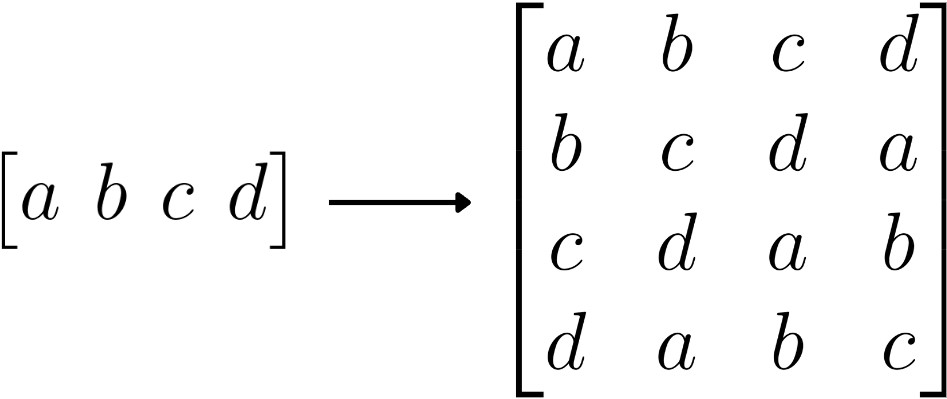
\includegraphics[width=0.4\linewidth]{Pictures/CNN_Model/string_conversion.jpg}
    \caption{Converting text to 2D text matrix}\label{fig:convert_text_img}
\end{figure}  

Note that this conversion depends on the length of the string 
used, i.e.\ for a string for length $n$, we will generate a 
$n \times n$ matrix. After we generate all variable-sized matrices, 
we resize them to $64 \times 64$ using Bilinear Interpolation.

Now we can see that a kernel (say $3 \times 3$ with stride one) 
can observe its previous as well as its next two characters and can 
use that information to find patterns in the ciphertext.

We use a CNN to extract features from the matrix and then we 
feed those features to a Dense Network to classify between the 
ciphertext types~\cite{DBLP:journals/corr/OSheaN15}.

\subsection{Motivation Behind Choosing Transformer Model}  

In our case, we used pre-trained transformer models, which have been fine-tuned using our own dataset. This allowed us to leverage the powerful language understanding capabilities of the transformer architecture while also ensuring that the model was specifically tailored to our problem.

The transformer architecture is based on the idea of self-attention, which allows the model to weigh the importance of different tokens in the input sequence when making predictions~\cite{vaswani2017attention}. This is done by computing a dot product between the input tokens and a set of learnable parameters, which are then used to generate a weight for each token. These weights are then used to compute a weighted average of the input tokens, which is used as the input to the next layer of the model.

This self-attention mechanism allows the transformer to effectively capture long-range dependencies between tokens, which is crucial for understanding the relationship between the ciphertext and the algorithm used to generate it. 

In summary, we have used the transformer model as it is a state-of-the-art model for sequence-to-sequence problems and its self-attention mechanism and multi-head attention allow the model to capture long-range dependencies between tokens and attend to different parts of the input sequence in parallel, which is crucial for understanding the relationship between the cipher-text and the algorithm used to generate it. 

\subsection{Transformer Based Proposed Model}  

The Transformer in NLP is a novel architecture that aims to 
solve sequence-to-sequence tasks while handling long-range dependencies 
with ease. The Transformer was proposed in the paper Attention 
Is All You Need~\cite{vaswani2017attention}. The main intuition behind this method is to compute the relative 
importance of a ciphertext character with respect to the other 
ciphertext characters. 

Our dataset contains encrypted 
text and the algorithm used for encryption, we create a text 
prompt from each row for example: 

\begin{flushleft}
    Cipher text: \texttt{ymccaygimgamkyyiycuycqocyeagmigkycmyyoyy}\\
    Algorithm: \texttt{affine}
\end{flushleft}  

The model learns the relative importance of each token (character) and uses 
it to predict the type of ciphertext. For example, if the model is trained 
with the above prompt and then we supply the following prompt: 

\begin{flushleft}
    Cipher text: \texttt{yycmdkreqluithnalekstndonwothvn}\\
    Algorithm: 
\end{flushleft}  

The model may generate the output as “affine” which it learned 
from training. 

In our use case, we have used the GPT-Neo (Generative Pre-Trained)~\cite{GPTNeo70:online}, 
a model with 125 million parameters to achieve our objective.  
It consists of a set of encoders and decoders placed one after 
the other. It has been pre-trained on Wikipedia Corpus ~\cite{EnglishC48:online}
and Common Crawl~\cite{CommonCr20:online} (This includes 12 years of data uploaded on the internet and has a size of over 12 Petabytes).
The word "Generative" suggests that the model is capable of text generation. The architecture is an extension to GPT2~\cite{radford2019language}. GPT-Neo~\cite{GPTNeo70:online} 
uses local attention in every other layer with a window size 
of 256 tokens. All these models are available for free in the 
Hugging Face \cite{HuggingF50:online} transformers library which can be used for a 
variety of NLP tasks.  

The following steps were taken for this model:
\begin{enumerate}
    \item   Each data is converted into text prompts 
            that is passed through a tokenizer that creates embedding 
            for each token in our input string. 
    \item   The input dataset has been split into the ratio 
            80:10:10 for training, testing, and validating purposes.
    \item   The training and validation set has been used to 
            fine-tune the model’s hyperparameters specific to 
            our use-case i.e. detecting the algorithm used in 
            the ciphertext generation.
    \item   We used the fine-tuned model on our test dataset 
            to check the accuracy of our model. 
    \item   After fine-tuning, for each of our test data we performed sampling with the temperature set to 0.7 to return 10 predictions. The maximum predicted algorithm is chosen to be the correct one and is then compared with the actual value to compute the accuracy.
\end{enumerate}  

For our testing purpose, we used various decoding strategies to find the one which gives the best result. Out of the strategies: Greedy Search, Beam Search and Sampling with set temperature, we found sampling  to give the most accurate results of all three. It is a method that is in between the greedy and sampling approach. 

The greedy method selects the next token that has the highest probability as the output while sampling selects one of the possible next tokens randomly. When we set a temperature, the randomness is lowered such that the likelihood of high-probability words is increased and that of the low probability is decreased. We found that a temperature set to 0.7 gave the optimum accuracy on our test data. 10 predictions are computed for each test data and the maximum predicted algorithm is chosen to be the correct one and is then compared with the actual value to compute the accuracy.

\begin{figure}
    \centering
    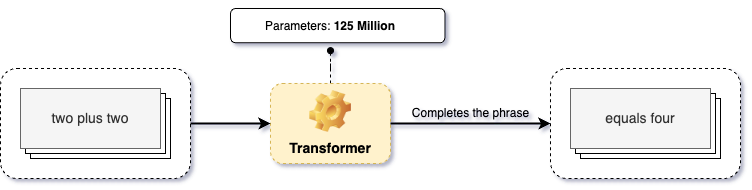
\includegraphics[width=\textwidth]{Pictures/pre-training.png}
    \caption{Pre-training}
    \label{fig2:preTraining}
    \hfill
\end{figure}

\begin{figure}
    \centering
    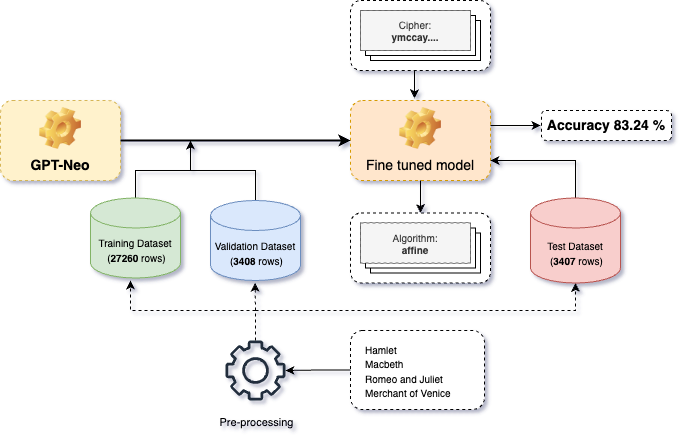
\includegraphics[width=\textwidth]{Pictures/fine-tuning.png}
    \caption{Fine-tuning}
    \label{fig3:fineTuning}
    \hfill
\end{figure}



\newpage
\section{Experimental Results}

\subsection{Dataset-1}

Our initial dataset consisted of 34075 rows that were split for training, testing, and validating in the ratio 80:10:10. The following are the sizes for each split:

\begin{itemize}
    \item Train dataset: 27260 rows
    \item Validation dataset: 3408 rows
    \item Test dataset: 3407 rows
\end{itemize}  

The following are the results obtained: 

\begin{table}[h!]
    \centering
    \caption{Training time and accuracy on Dataset-1}
    \begin{tabular}{|c|c|c|c|}
    \hline
         \bfseries Model & \bfseries Number of Classes & \bfseries Training time & \bfseries Accuracy \\
    \hline
         CNN(125M) & 5 & 48 mins & 60.12\% \\
    \hline
         GPT-Neo(125M) & 5 & 37 mins & 83.24\% \\
    \hline
         OPT(125M) & 5 & 34 mins & 85.29\% \\
    \hline
    \end{tabular}
    \label{tab:dataset-1}
\end{table}  

% \begin{figure}
% \includegraphics[width=0.6\linewidth]{Graphs/accuracy-dataset-1.eps}
% \includegraphics[width=0.6\linewidth]{Graphs/training-time-dataset-1.eps}
% \label{fig2}
% \end{figure}

\begin{figure}
    \centering
    \begin{subfigure}[b]{0.495\textwidth}
        \centering
        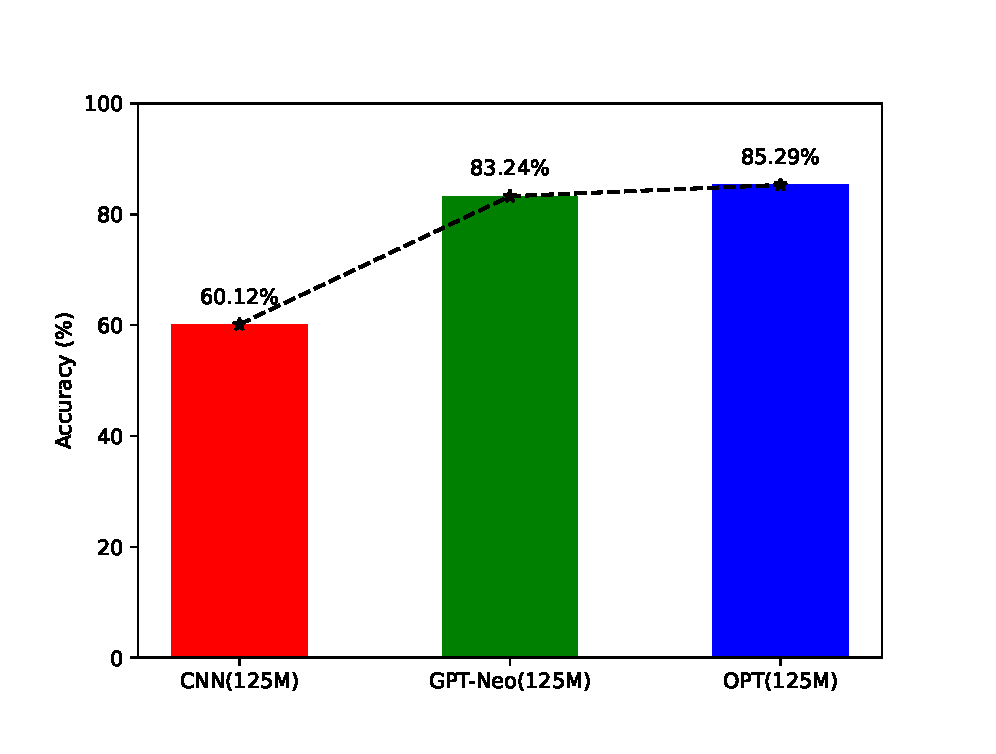
\includegraphics[width=\textwidth]{Pictures/Graphs/accuracy-dataset-1.eps}
        \caption{Accuracy}
        \label{fig4.1:dataset1Accuracy}
    \end{subfigure}
    \hfill
    \begin{subfigure}[b]{0.495\textwidth}
        \centering
        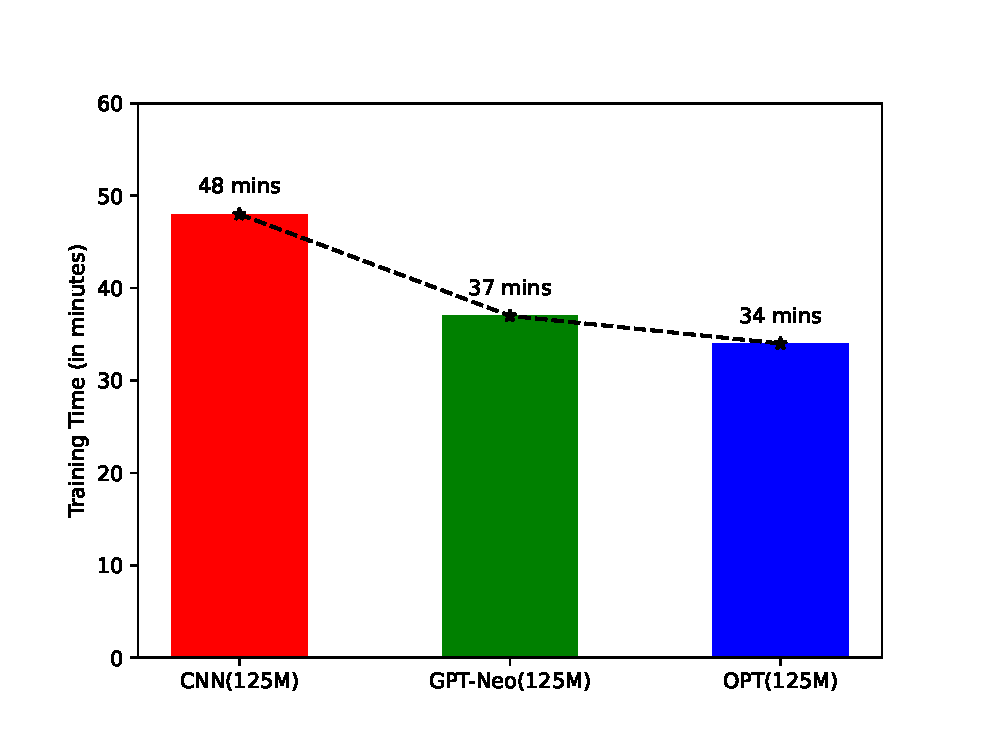
\includegraphics[width=\textwidth]{Pictures/Graphs/training-time-dataset-1.eps}
        \caption{Training Time}
        \label{fig4.2:dataset1TrainaingTime}
    \end{subfigure}
       \caption{Comparison of Accuracies and Training Times on Dataset 1}
       \label{fig4:dataset1Result}
\end{figure}

\subsection{Dataset-2} 


Next, we increased our dataset containing  133880 rows that were split for training, testing, and validating in the ratio 80:10:10. The following are the sizes for each split:  

\begin{itemize}
    \item Train dataset: 107104 rows
    \item Validation dataset: 13388 rows
    \item Test dataset: 13388 rows
\end{itemize}  

The following are the results obtained: 

\begin{table}[h!]
    \centering
    \caption{Training time and accuracy on Dataset-2}
    \begin{tabular}{|c|c|c|c|}
    \hline
         \bfseries Model & \bfseries Number of Classes & \bfseries Training time & \bfseries Accuracy \\
    \hline
         CNN(125M) & 5 & 5 hrs 10 mins & 69.01\% \\
    \hline
         GPT-Neo(125M) & 5 & 2 hrs 39 mins & 90.61\% \\
    \hline
         OPT(125M) & 5 & 2 hrs 31 mins & 96.72\% \\
    \hline
    \end{tabular}
    \label{tab:dataset-2}
\end{table} 

% \begin{figure}
% \includegraphics[width=0.6\linewidth]{Graphs/accuracy-dataset-2.eps}
% \includegraphics[width=0.6\linewidth]{Graphs/training-time-dataset-2.eps}
% \label{fig2}
% \end{figure}

\begin{figure}
    \centering
    \begin{subfigure}[b]{0.495\textwidth}
        \centering
        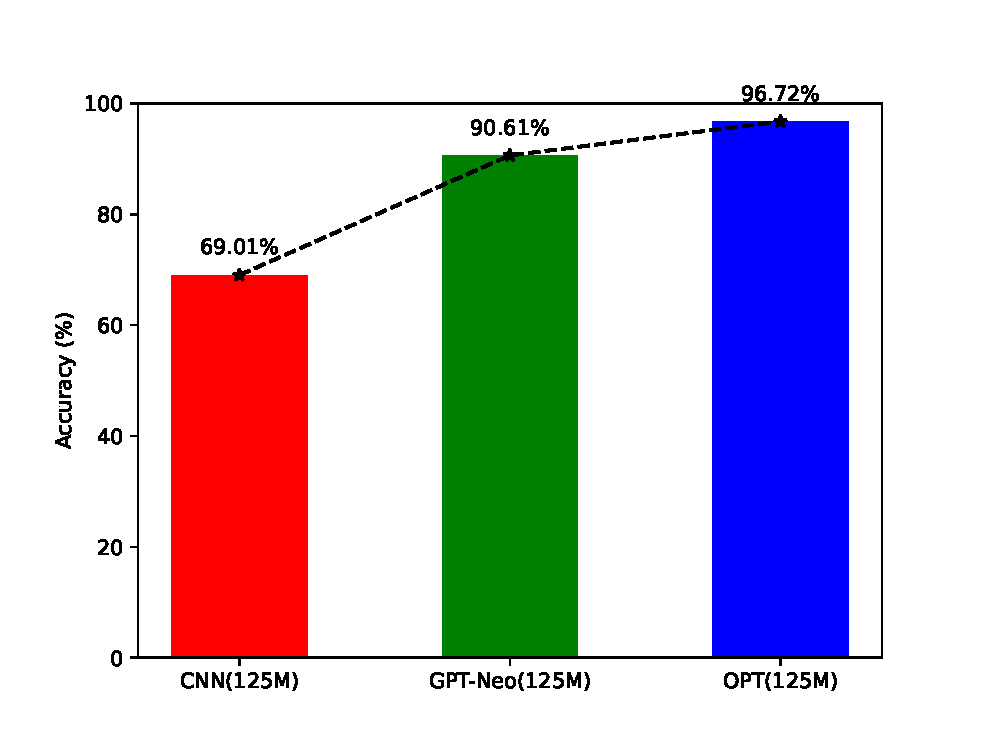
\includegraphics[width=\textwidth]{Pictures/Graphs/accuracy-dataset-2.eps}
        \caption{Accuracy}
        \label{fig5.1:dataset2Accuracy}
    \end{subfigure}
    \hfill
    \begin{subfigure}[b]{0.495\textwidth}
        \centering
        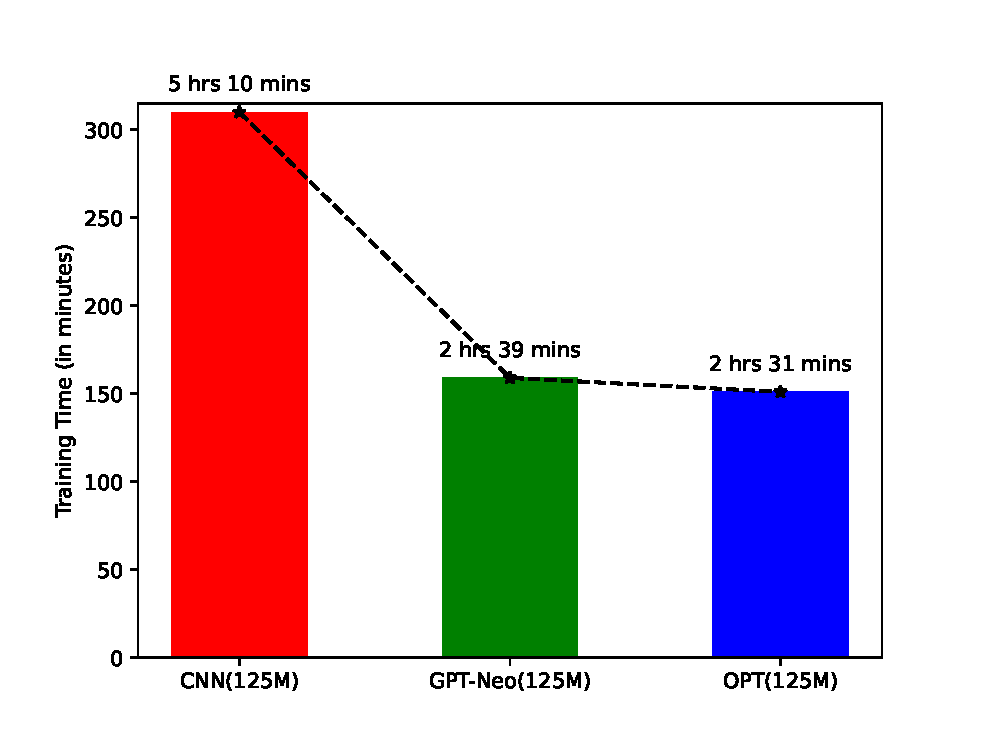
\includegraphics[width=\textwidth]{Pictures/Graphs/training-time-dataset-2.eps}
        \caption{Training Time}
        \label{fig5.2:dataset2TrainaingTime}
    \end{subfigure}
       \caption{Comparison of Accuracies and Training Times on Dataset 2}
       \label{fig5:dataset2Result}
\end{figure}

\section{Conclusion}

This paper shows the current progress of our work in the detection of ciphertext using Artificial Neural Networks. Here we used three types of Neural Networks to achieve our objective, namely: Convolution Neural Networks and GPT-Neo and OPT. 

With the CNN approach, our model was able to achieve an accuracy of 68.30\% for 5 class classifications. We saw a significant improvement with the transformers approach using GPT-Neo on the same dataset and classes giving an accuracy of 90.61\%. This was primarily due to the ability of GPT-Neo to memorize the local importance of tokens due to the self-attention feature. OPT gave better improvements, giving an accuracy of 96.72\%, signifying that OPT is better than GPT-Neo for the task of detecting the type of ciphertext. We also observed that transformer based models are giving better result than CNN while taking less time for training.

In future work, we will use similar transformer based model like BERT, GPTJ and Bloom to see if those models are better suited for the task. We will also extend the number of classes of ciphertext and size of dataset to see if we observe any improvements.

% ---- Extras ----

% \paragraph{Sample Heading (Fourth Level)}
% The contribution should contain no more than four levels of
% headings. Table~\ref{tab1} gives a summary of all heading levels.

% \begin{table}
% \caption{Table captions should be placed above the
% tables.}\label{tab1}
% \begin{tabular}{|l|l|l|}
% \hline
% Heading level &  Example & Font size and style\\
% \hline
% Title (centered) &  {\Large\bfseries Lecture Notes} & 14 point, bold\\
% 1st-level heading &  {\large\bfseries 1 Introduction} & 12 point, bold\\
% 2nd-level heading & {\bfseries 2.1 Printing Area} & 10 point, bold\\
% 3rd-level heading & {\bfseries Run-in Heading in Bold.} Text follows & 10 point, bold\\
% 4th-level heading & {\itshape Lowest Level Heading.} Text follows & 10 point, italic\\
% \hline
% \end{tabular}
% \end{table}
% \noindent Displayed equations are centered and set on a separate
% line.
% \begin{equation}
% x + y = z
% \end{equation}
% Please try to avoid rasterized images for line-art diagrams and
% schemas. Whenever possible, use vector graphics instead (see
% Fig.~\ref{fig1}).

% \begin{figure}
% \includegraphics[width=\textwidth]{fig1.eps}
% \caption{A figure caption is always placed below the illustration.
% Please note that short captions are centered, while long ones are
% justified by the macro package automatically.} \label{fig1}
% \end{figure}

% \begin{theorem}
% This is a sample theorem. The run-in heading is set in bold, while
% the following text appears in italics. Definitions, lemmas,
% propositions, and corollaries are styled the same way.
% \end{theorem}
% %
% % the environments 'definition', 'lemma', 'proposition', 'corollary',
% % 'remark', and 'example' are defined in the LLNCS documentclass as well.
% %
% \begin{proof}
% Proofs, examples, and remarks have the initial word in italics,
% while the following text appears in normal font.
% \end{proof}
% For citations of references, we prefer the use of square brackets
% and consecutive numbers. Citations using labels or the author/year
% convention are also acceptable. The following bibliography provides
% a sample reference list with entries for journal
% articles~\cite{ref_article1}, an LNCS chapter~\cite{ref_lncs1}, a
% book~\cite{ref_book1}, proceedings without editors~\cite{ref_proc1},
% and a homepage~\cite{ref_url1}. Multiple citations are grouped
% \cite{ref_article1,ref_lncs1,ref_book1},
% \cite{ref_article1,ref_book1,ref_proc1,ref_url1}.
%
% ---- Bibliography ----
%
% BibTeX users should specify bibliography style 'splncs04'.
% References will then be sorted and formatted in the correct style.
%
\bibliographystyle{splncs04}
\bibliography{mp}
\end{document}